%$Id: qrezix.tex 144 2005-03-25 01:11:37Z myk $

\subsection{La t�l�vision du BR}
\label{TV}

Le BR diffuse sur le r�seau sept chaines de t�l�vision et une vingtaine de radios. Pour les recevoir, nous recommandons \app{vlc}, disponible sur le X-Share.

\subsubsection{Configuration de \app{vlc}}

La liste des chaines est diffus�e sous forme d'annonces SAP. Pour voir ces annonces, ouvre ta liste de lecture (Vue -> Liste de lecture), et active la decouverte de services.

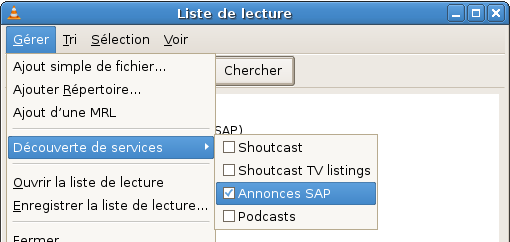
\includegraphics[width=0.7\textwidth]{images/vlc_config_sap.png}

Tu auras ainsi dans ta liste de lecture les diff�rents chaines disponibles.

\subsubsection{Autre m�thode}

Si ton client pr�f�r� ne supporte pas les annonces SAP, ou que les annonces SAP ne marchent pas chez toi, tu peux r�cup�rer la liste des chaines par
PodCast, � l'adresse \url{http://tv.eleves.polytechnique.fr/tvbr.xml}. Sous \app{vlc}, active la d�couverte des services PodCast dans la liste de
lecture (G�rer > D�couverte de services > Podcast), puis va dans Param�tres > Pr�f�rences > Liste de Lecture > D�couverte de services > Podcast et
met l'adresse \url{http://tv.eleves.polytechnique.fr/tvbr.xml} dans le champ \guillemotleft~Liste des URLs~\guillemotright .

\subsubsection{Et si �a ne marche toujours pas?}

V�rifie que tu utilises bien la derni�re version de \app{vlc}. Les versions inf�rieures � 0.8.5 sont connues pour ne pas fonctionner.

Si rien ne marche, la raison la plus probable est un \emph{firewall} qui intercepte les flux t�l�s. Configure ton \emph{firewall} afin d'autoriser
ces flux. Sous Linux, les r�gles \emph{iptables} suivantes suffisent:

  \cmdline[0.85] {
   -A INPUT -i eth0 -d 224.0.0.0/24 -j ACCEPT
   -A INPUT -i eth0 -d 239.255.42.0/24 -s 192.168.225.0/24 -p udp -m udp --dport 1234 -j ACCEPT
   -A INPUT -i eth0 -d 239.255.255.255/32 -p udp -m udp --dport 9875 -j ACCEPT
   -A OUTPUT -o eth0 -d 224.0.0.0/4 -j ACCEPT.
  }
